\documentclass[a4paper]{article}
\usepackage[margin=0.5in]{geometry}
%\usepackage{fontspec}


%%%%lualatex on
%\usepackage{luatextra}
\usepackage{fontspec}
\usepackage{todonotes}
%Ligatures={Contextual, Common, Historical, Rare, Discretionary}
\setmainfont[Mapping=tex-text]{Apple Garamond}
%%First draft of a research proposal

\usepackage{natbib}
\usepackage{graphicx}


\title{notes}
\author{Simon Carrignon}

\begin{document}
Le model se decline en deux version:

\begin{itemize}
    \item Une version dans laquelle les agents doivent se mettre d accords sur les prix de sorte a ce que tous puisse recuperer les mêmes quantités de chaque bien
    \item Une verison dans laquelle  les agents doivent se emttre d'accords sur des prix qui permettent à tous de maximiser leur fonction d'utilité (unique)
\end{itemize}

	%%\includegraphics[width=.8\textwidth]{../images/RandRvsRandom100Agents4goods.pdf}\\  All those image are deleted as they where showing result using a bad social learning mechanism
	%%\includegraphics[width=.8\textwidth]{../images/RandRvsRandom200Agents4goods.pdf}\\
	%%\includegraphics[width=.8\textwidth]{../images/RandRvsRandom300Agents4goods.pdf}\\
	%%\includegraphics[width=.8\textwidth]{../images/RandRvsRandom400Agents4goods.pdf}\\
	%%\includegraphics[width=.8\textwidth]{../images/RandRvsRandom500Agents4goods.pdf}

	\begin{itemize}
	    \item  Social process: 
		\begin{itemize}
		    \item Social Learning
			\begin{itemize}
			    \item copymin : the is the one we use
			    \item copymax : should not change so much but eh ocnsumtion shoudl be diffiernt
			\end{itemize}
		    \item Innovation: random mutation $\mu$
		\end{itemize}
		
	z    \item  Economic process:
		\begin{itemize}
		    \item prices initialization:
			\begin{itemize}
			    \item gintis,
			    \item random= optimal price at the begining are U(0,1) 
			    \item randn= optimal price at the begining are normalised to ONE
			\end{itemize}
		    \item evaluation function: this should be the function that we somehow been used afterward by social process (copmin/copmax)
		    \item Exchange Rules 
			\begin{itemize}
			    \item Accept only the need and no more : $\leftarrow$ Do the comparaison because it would be better to NOT have that (avoid the use of the need when doing the exchange ie less information)
			\end{itemize}
		\end{itemize}
	\end{itemize}
	\section{Actual State of the model}
	After some years of fight, I finally go down to see who is buying to whom what and how. It allowed me to see one thing: A lot of transaction where not done due to stuff like:

	$$3==3 \Rightarrow FALSE$$

	that was du to double comparaison where indeed 
	$$3==3 \Leftrightarrow 3.00000123231 == 3.00000 \Rightarrow FALSE$$

	This led to another problem : what means ``similar/enough/not enough'' for our agents? That could/should be traited, and the amnagemetn of thisshould be traited by the agents themesleves (to allow different way of seeing that)

	As one can seen in the results of the figure~\ref{fig:eq}, the cultural operators are not starting at the first time step. It's not very usefull and could/should be remove, it was introduced more for debugging purpose.

	New features: \begin{description}
	    \item[Events] the environmentStep( )function, defined in World.cxx, as been rewrited in Province. This allowed us to introduce \emph{events}. So far they are really simple but shoudl be more parametrized in two way: Manually and auto. The manual mode will be used for the ICRATES data, the auto will be sued first for test entwork resiliences.
	    \item[mutation amplityutede] now in the config file one can not only define the probability of a mutation but also the \emph{amplitutde} of this mutation. \todo{this is not rely improving because the best way to do would be to integrate the mutation at the inovation process: \emph{ie} evolve the amplitude as it's done in Evolutionary Computation. This would mean that human aren't so stupid and mutation are \emph{guided}}
	    \item[trade culture]  listing of the diferent things implementend so far
		\begin{description}
		    \item[custom] notre belle fucntion
		    \item[gintis06] quantity/need
		\end{description}
	    \item[..] il en manque
	\end{description}
	
	\section{Actuals equilibrium}
	\subsection{maintaineing the equilibrum}

	In those experiments the goods start with their equilibrium prices but with 0 quantitites
	As we can see in the scores things there is 2 rounds of no inovation/copy



	%\begin{table}
	%    \centering
	%    \caption{Test with prices starting at their optimal values}
	%    \label{fig:eq}
	%    \begin{tabular}{llccc}
	%	Uitily & Trade &agents'score wrt tim &  Distance to ideal prices & distance to ideal quantities \\
	%	Custom & Need & 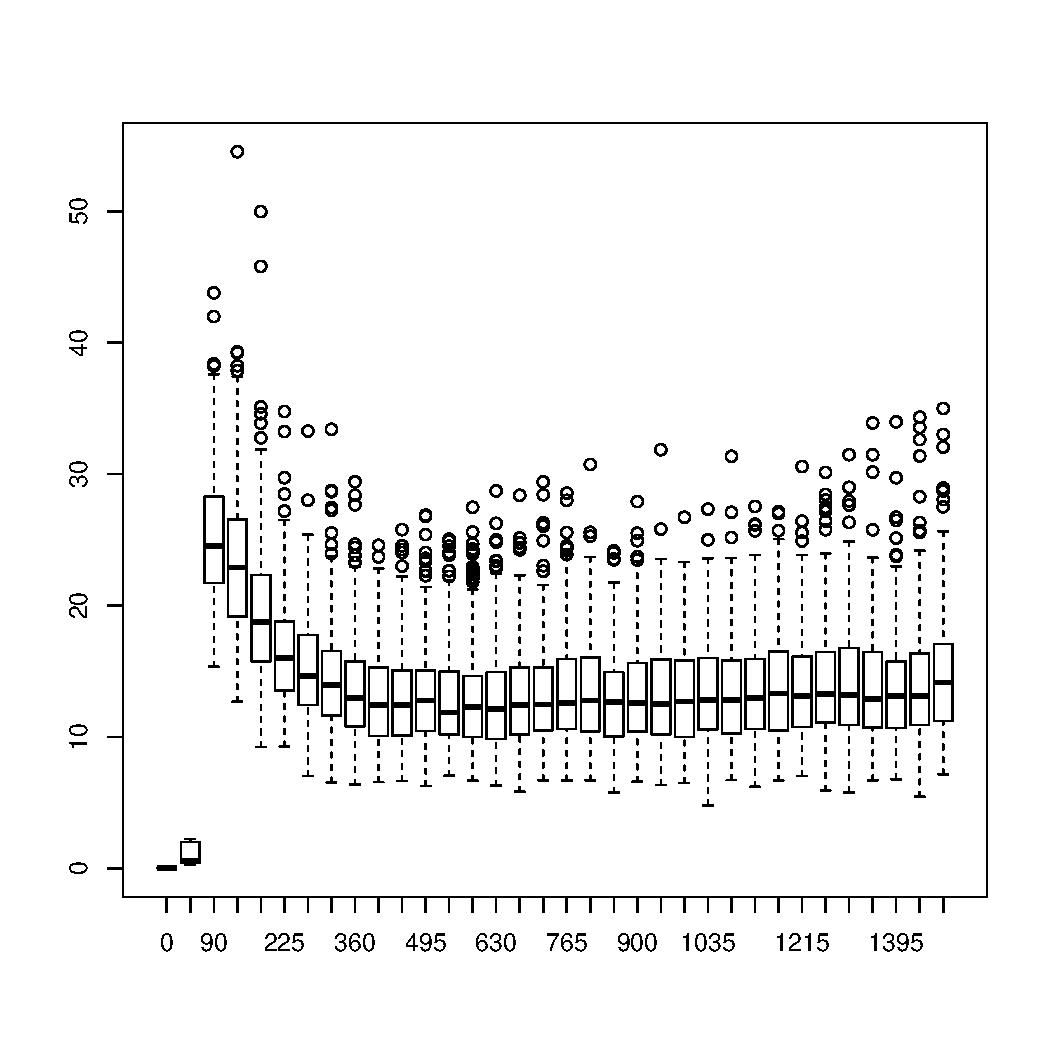
\includegraphics[width=.18\textwidth]{images/Scores-300Ag5goodmanualTradGintisTakingNeedAccountCustomUitiliy.pdf} & 
	%	\includegraphics[width=.18\textwidth]{images/Prices-300Ag5goodmanualTradGintisTakingNeedAccountCustomUitiliy.pdf} & 
	%	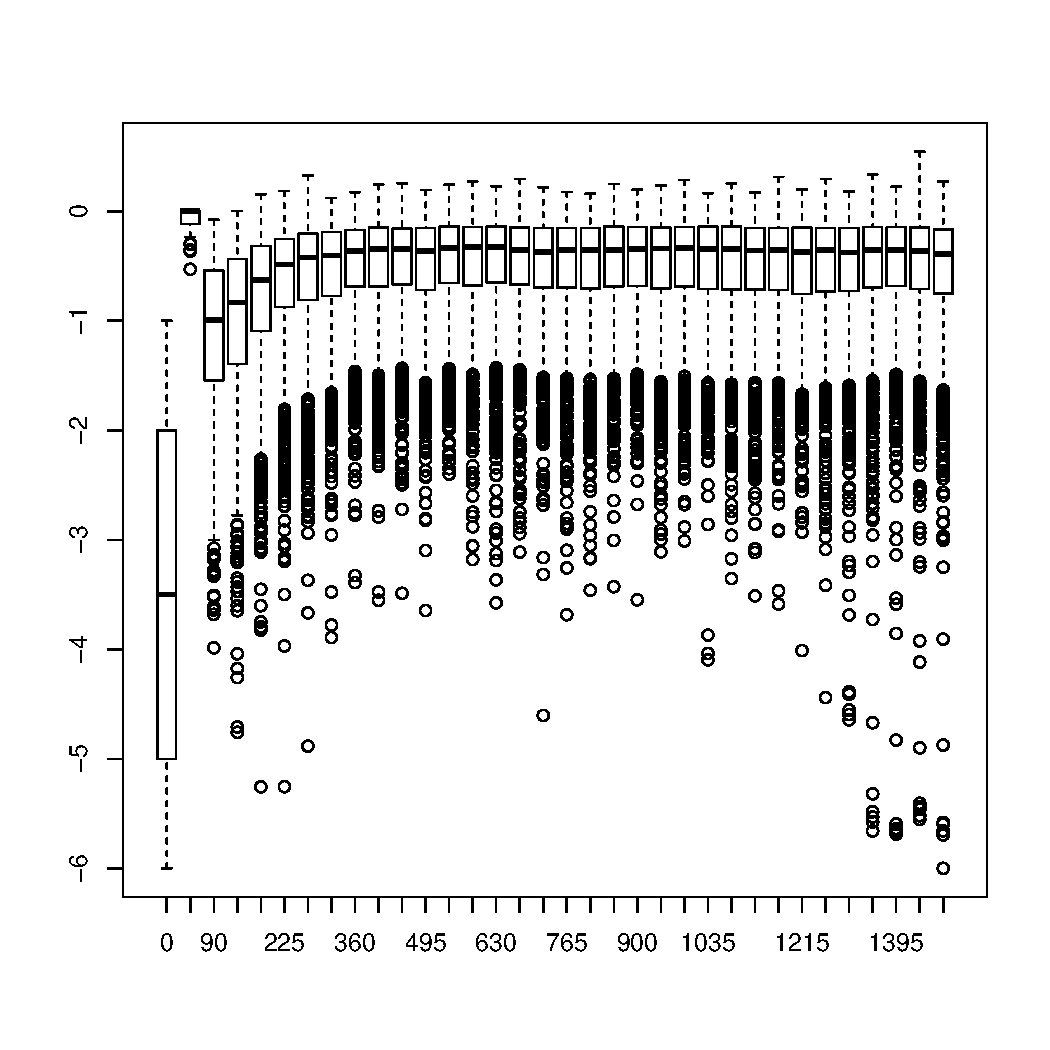
\includegraphics[width=.18\textwidth]{images/Quantities-300Ag5goodmanualTradGintisTakingNeedAccountCustomUitiliy.pdf} \\
	%	Custom & No Need & \includegraphics[width=.18\textwidth]{images/Scores-300Ag5goodmanualTradGintisTakingNoNeedAccountCustomUitiliy.pdf} & 
	%	\includegraphics[width=.18\textwidth]{images/Prices-300Ag5goodmanualTradGintisTakingNoNeedAccountCustomUitiliy.pdf} & 
	%	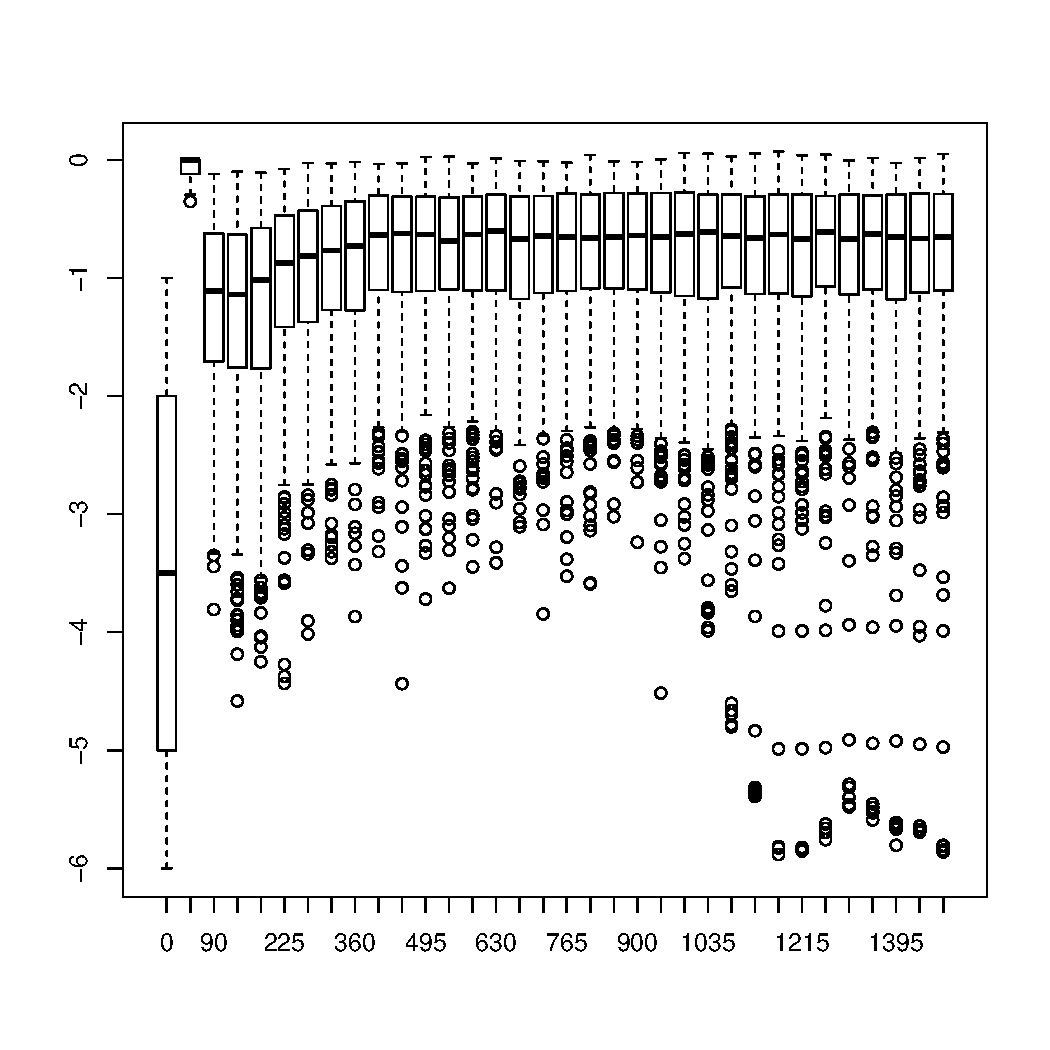
\includegraphics[width=.18\textwidth]{images/Quantities-300Ag5goodmanualTradGintisTakingNoNeedAccountCustomUitiliy.pdf} \\
	%	Gintis & No Need & 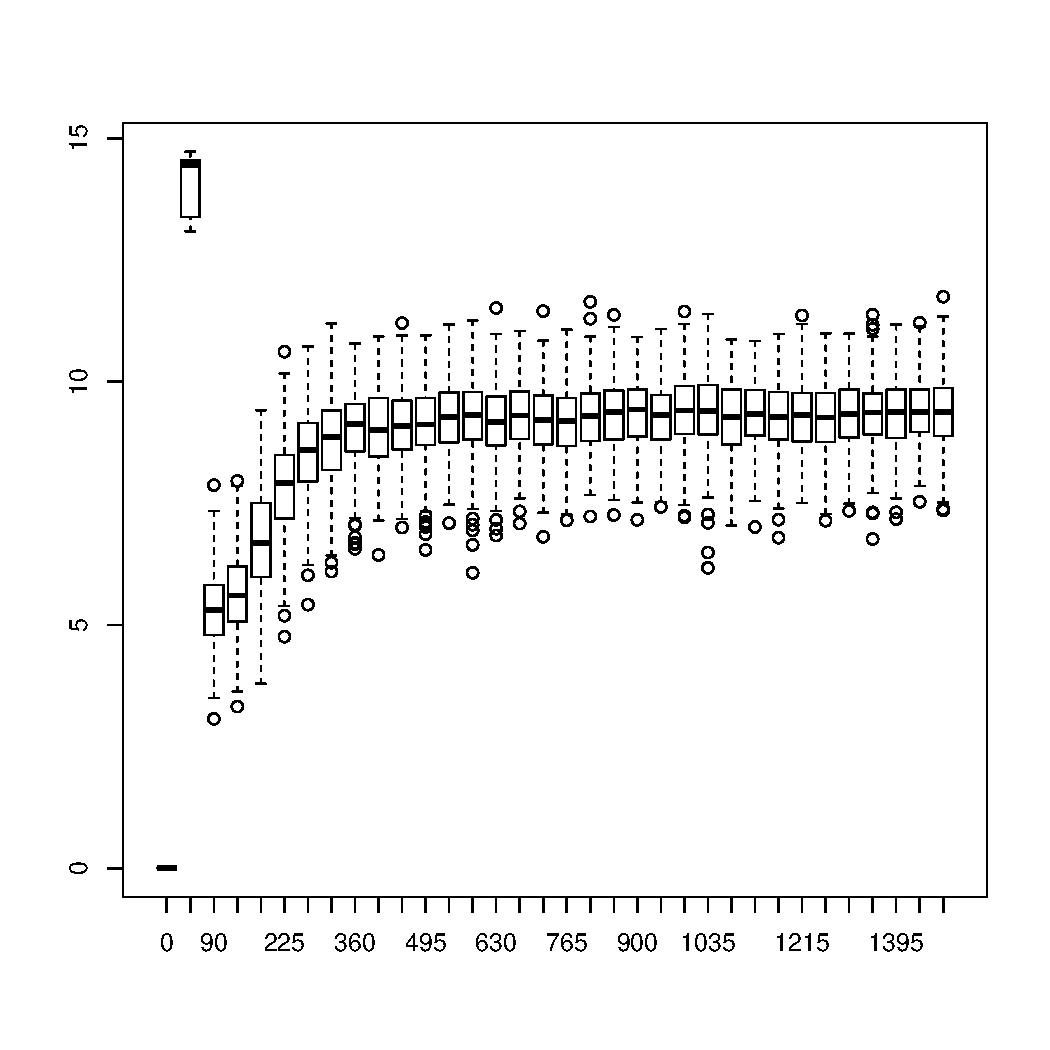
\includegraphics[width=.18\textwidth]{images/Scores-300Ag5goodmanualTradGintisTakingNoNeedAccountGintisUitiliy.pdf} & 
	%	\includegraphics[width=.18\textwidth]{images/Prices-300Ag5goodmanualTradGintisTakingNoNeedAccountGintisUitiliy.pdf} & 
	%	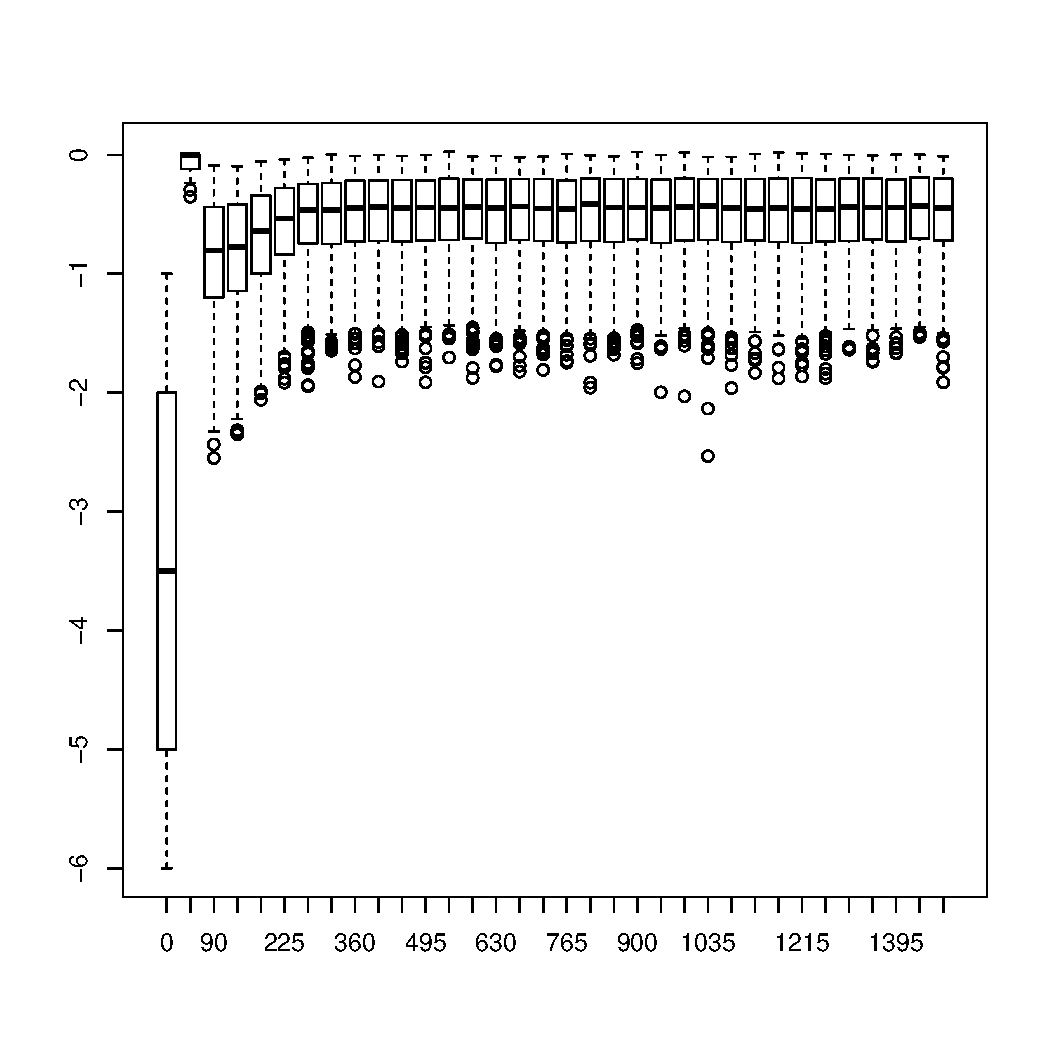
\includegraphics[width=.18\textwidth]{images/Quantities-300Ag5goodmanualTradGintisTakingNoNeedAccountGintisUitiliy.pdf} \\
	%	Gintis & Need & 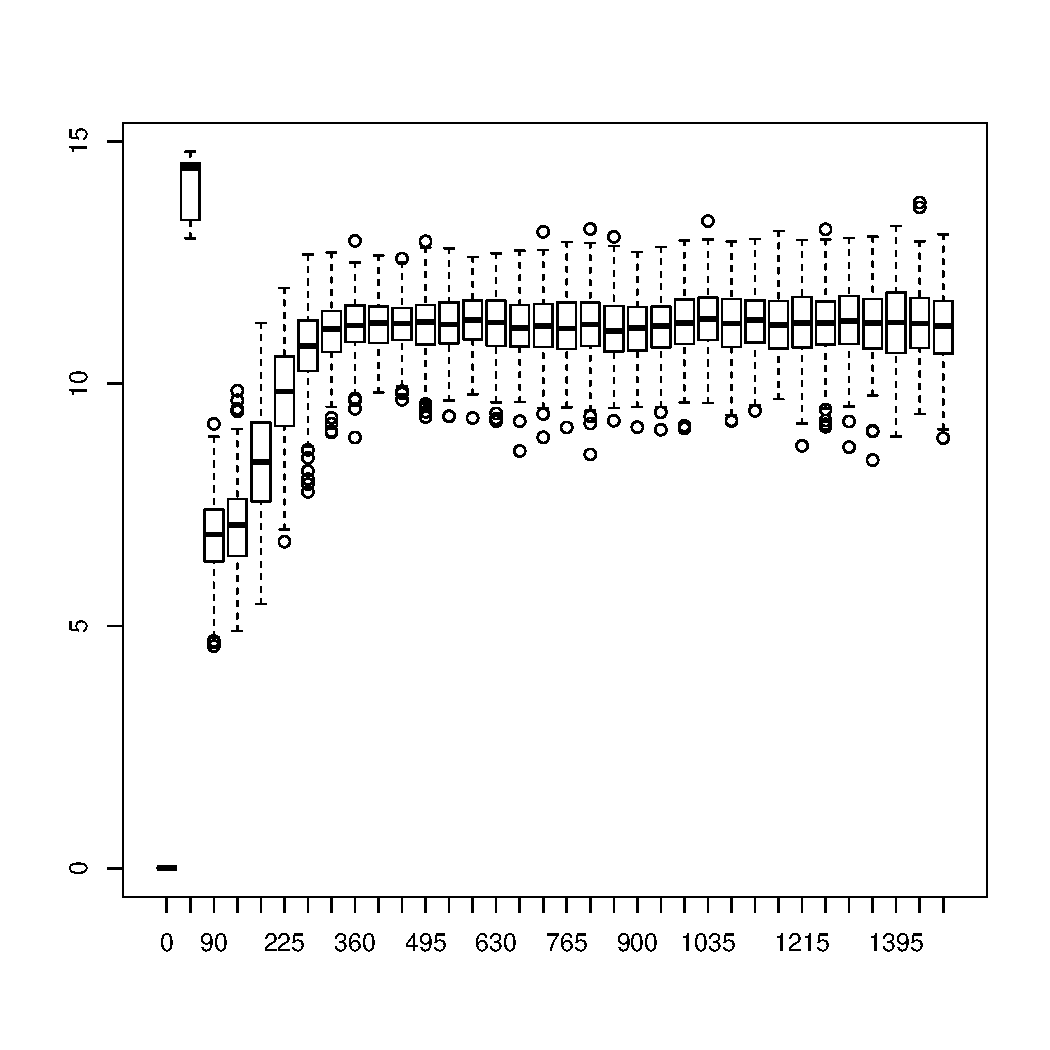
\includegraphics[width=.18\textwidth]{images/Scores-300Ag5goodmanualTradGintisTakingNeedAccountGintisUitiliy.pdf} & 
	%	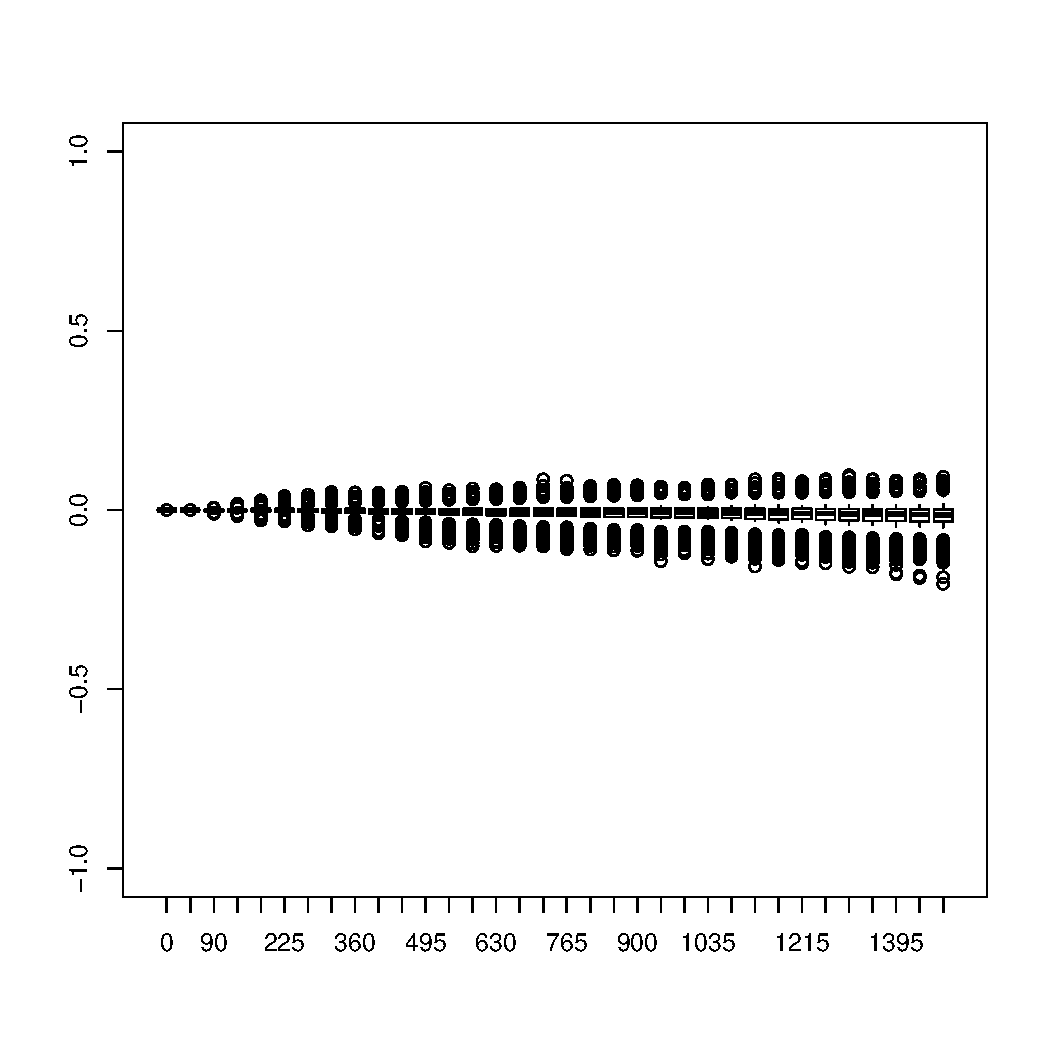
\includegraphics[width=.18\textwidth]{images/Prices-300Ag5goodmanualTradGintisTakingNeedAccountGintisUitiliy.pdf} & 
	%	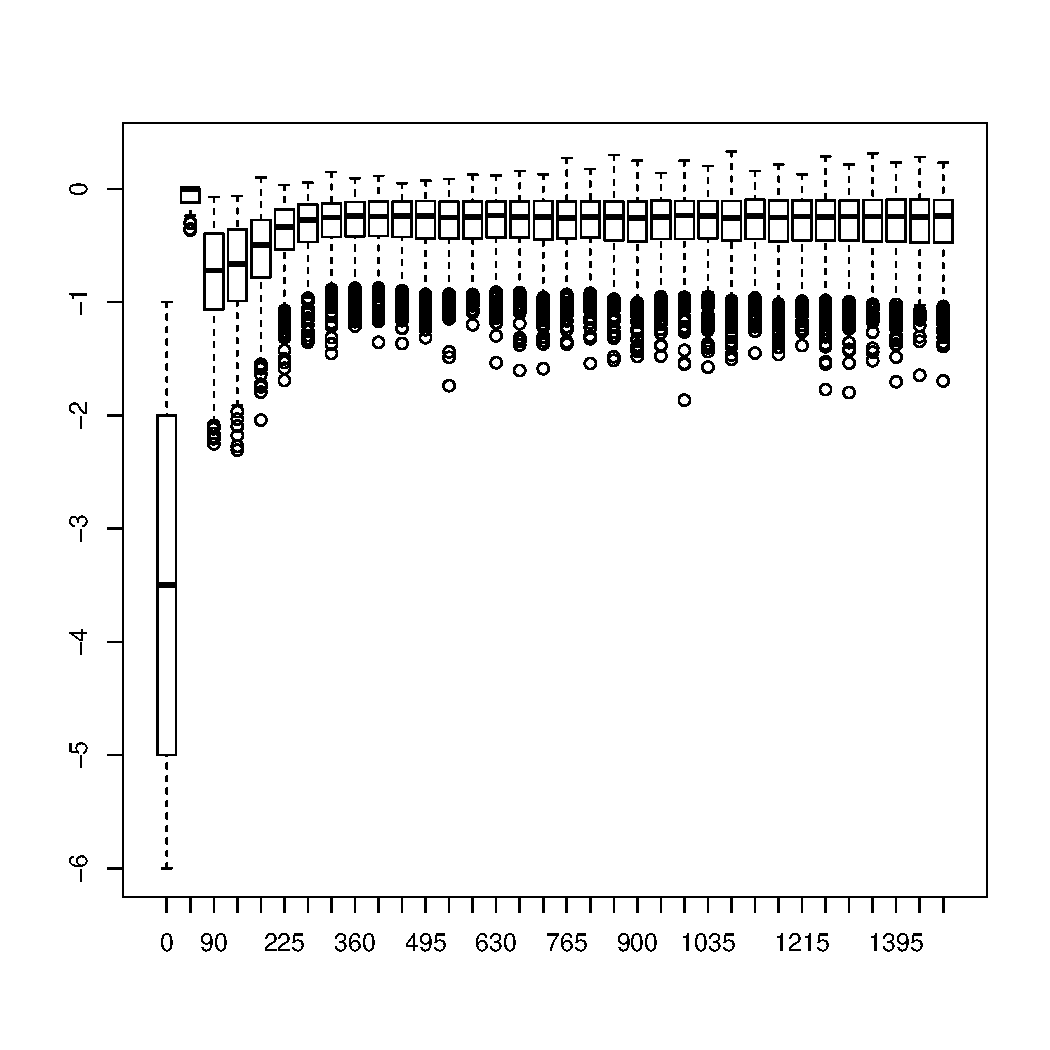
\includegraphics[width=.18\textwidth]{images/Quantities-300Ag5goodmanualTradGintisTakingNeedAccountGintisUitiliy.pdf} \\
	%    \end{tabular}
	%\end{table}
	We observe in that case that after few time step the different metrics go away from the optimal values: indeed, the aparation of the cultural mechanisms (inovationa dn copy)  add noise that prohibit all the agents to do the best move. \todo{Those result are not at the equilibrium: it's seems that it is still divereigng: when maresnostrum's back: run longer time}


	\subsection{finding the equilibrum}

	Same than before bust this time the price of goods at the beginning \emph{is not} set as it optimal value
	In both following cases the importance of the amplitutde of the mutation is really important:
		\begin{itemize}
		    \item If needs  are $> 1$ then the prices will be $\in [0,1]$
		    \item If needs  are $\in [0,1]$ then prices can easily scale up to $+\infty$

		\end{itemize}

	\subsubsection{With need normalized: $\sum{needs}=1$}
		


	\begin{table}
	    \centering
	    \begin{tabular}{llccc}
		Uitily & Trade &agents'score wrt tim &  Distance to ideal prices & distance to ideal quantities \\
		%Custom & Need & \includegraphics[width=.18\textwidth]{images/Scores-300Ag5goodrandnTradGintisTakingNeedAccountCustomUitiliy.pdf} & 
		%%\includegraphics[width=.18\textwidth]{images/Prices-300Ag5goodrandnTradGintisTakingNeedAccountCustomUitiliy.pdf} & 
		%%\includegraphics[width=.18\textwidth]{images/Quantities-300Ag5goodrandnTradGintisTakingNeedAccountCustomUitiliy.pdf} \\
		%%Custom & No Need & \includegraphics[width=.18\textwidth]{images/Scores-300Ag5goodrandnTradGintisTakingNoNeedAccountCustomUitiliy.pdf} & 
		%%\includegraphics[width=.18\textwidth]{images/Prices-300Ag5goodrandnTradGintisTakingNoNeedAccountCustomUitiliy.pdf} & 
		%%\includegraphics[width=.18\textwidth]{images/Quantities-300Ag5goodrandnTradGintisTakingNoNeedAccountCustomUitiliy.pdf} \\
		Gintis & No Need & \includegraphics[width=.18\textwidth]{images/Scores-300Ag5goodrandnTradGintisNoNeedAccountGintisUitiliy.pdf} & 
		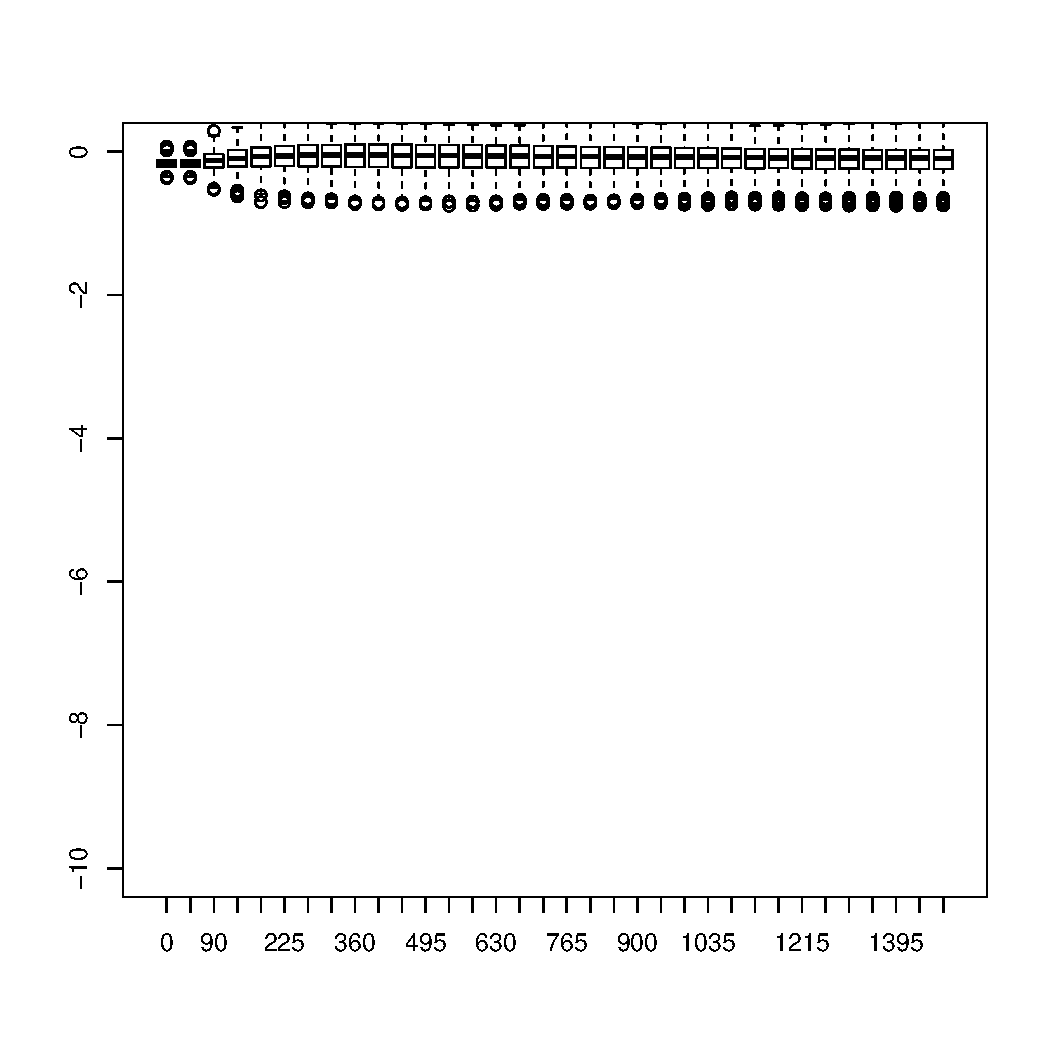
\includegraphics[width=.18\textwidth]{images/Prices-300Ag5goodrandnTradGintisNoNeedAccountGintisUitiliy.pdf} & 
		\includegraphics[width=.18\textwidth]{images/Quantities-300Ag5goodrandnTradGintisNoNeedAccountGintisUitiliy.pdf} \\
		Gintis & Need & 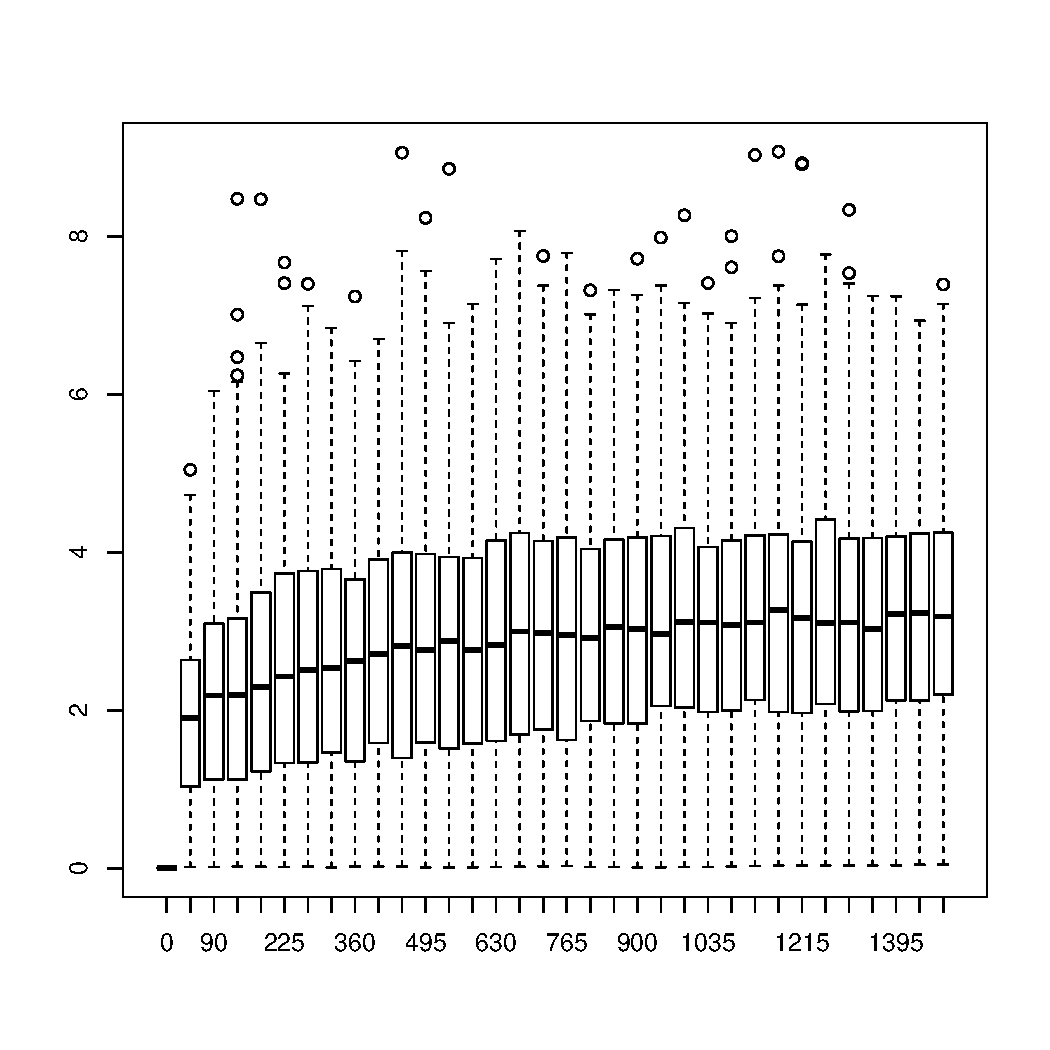
\includegraphics[width=.18\textwidth]{images/Scores-300Ag5goodrandnTradGintisTakingNeedAccountGintisUitiliy.pdf} & 
		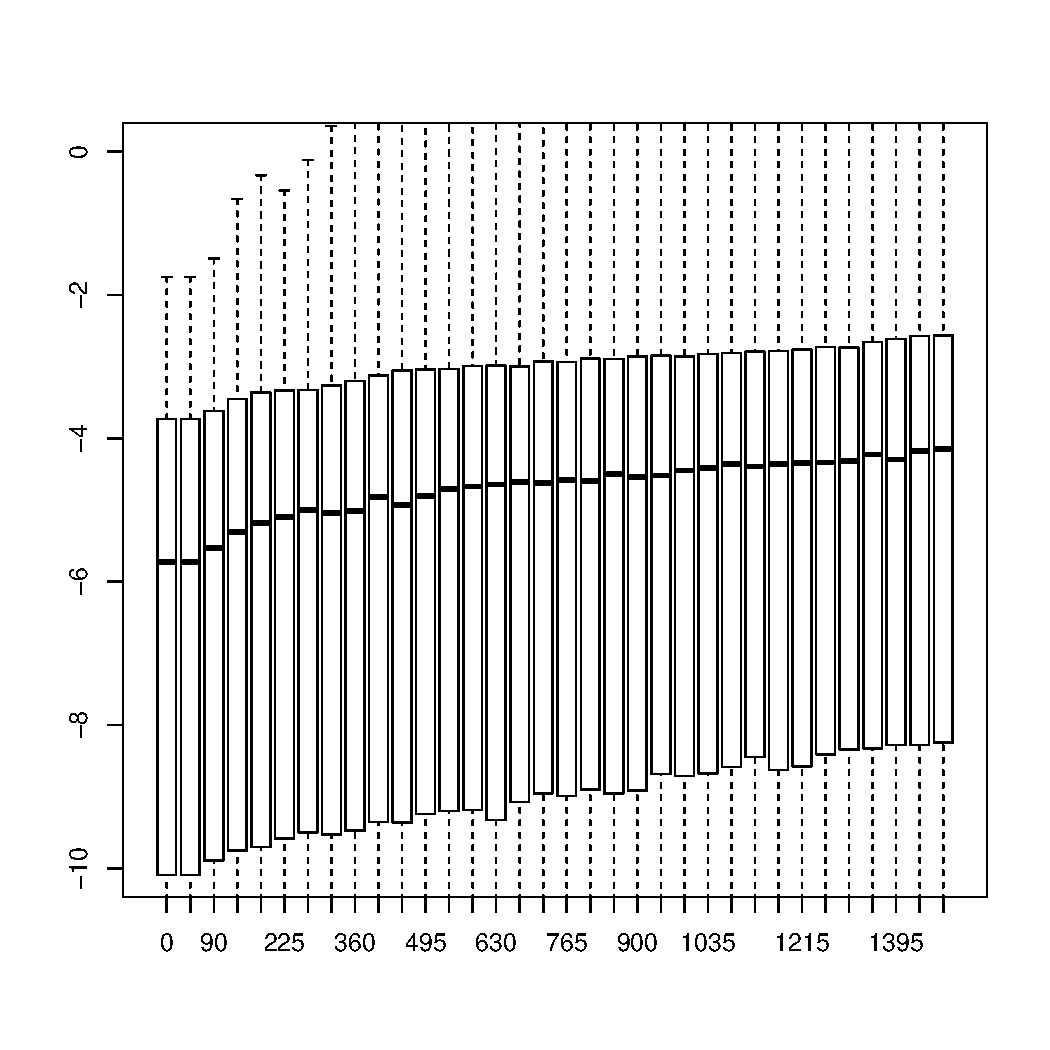
\includegraphics[width=.18\textwidth]{images/Prices-300Ag5goodrandnTradGintisTakingNeedAccountGintisUitiliy.pdf} & 
		\includegraphics[width=.18\textwidth]{images/Quantities-300Ag5goodrandnTradGintisTakingNeedAccountGintisUitiliy.pdf} \\
	    \end{tabular}
	\end{table}




\begin{table}[ht]
\centering
\begin{tabular}{lllllll}
  \hline
Copy & Init & Choice & Util & Scores & Prices & Quantities \\ 
  \hline
prod & man & gin & cust & \includegraphics[width=.18\textwidth]{/home/scarrign/projects/PhD/doc/thesis/images/Scores-1_cult-prod_init-man_volsel-gin_ufun-cust.pdf} & 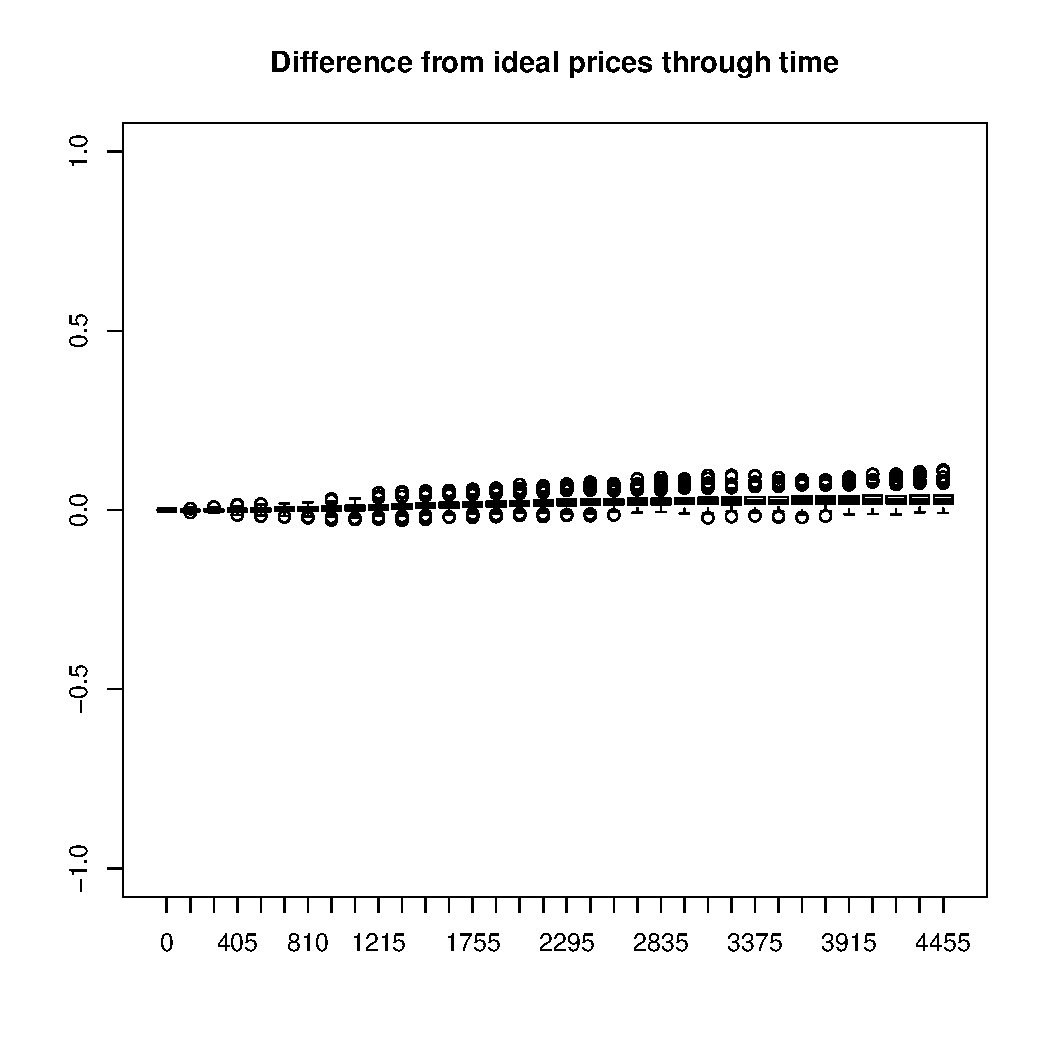
\includegraphics[width=.18\textwidth]{/home/scarrign/projects/PhD/doc/thesis/images/Prices-1_cult-prod_init-man_volsel-gin_ufun-cust.pdf} & \includegraphics[width=.18\textwidth]{/home/scarrign/projects/PhD/doc/thesis/images/Quantities-1_cult-prod_init-man_volsel-gin_ufun-cust.pdf} \\ 
  prod & man & gin & gin & 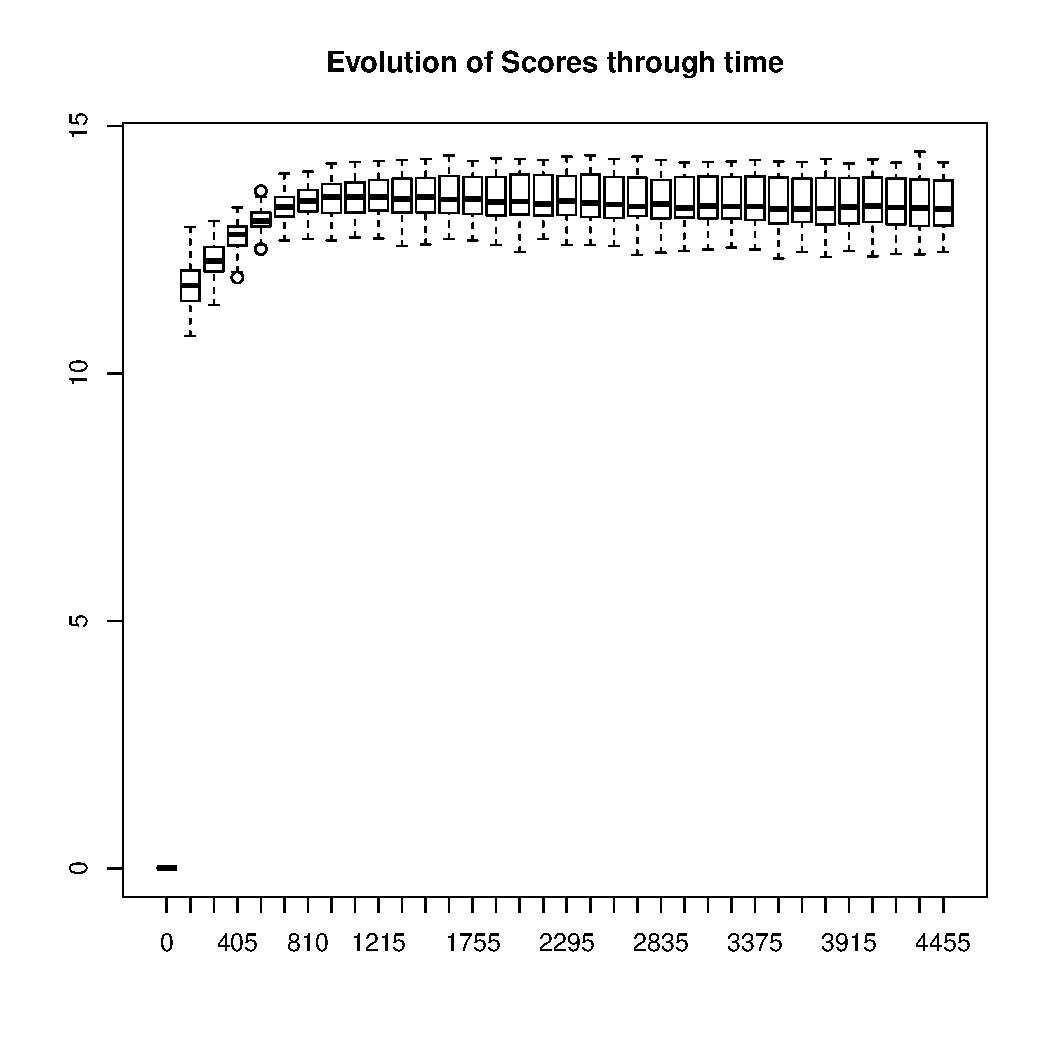
\includegraphics[width=.18\textwidth]{/home/scarrign/projects/PhD/doc/thesis/images/Scores-2_cult-prod_init-man_volsel-gin_ufun-gin.pdf} & \includegraphics[width=.18\textwidth]{/home/scarrign/projects/PhD/doc/thesis/images/Prices-2_cult-prod_init-man_volsel-gin_ufun-gin.pdf} & \includegraphics[width=.18\textwidth]{/home/scarrign/projects/PhD/doc/thesis/images/Quantities-2_cult-prod_init-man_volsel-gin_ufun-gin.pdf} \\ 
  prod & man & gino & cust & \includegraphics[width=.18\textwidth]{/home/scarrign/projects/PhD/doc/thesis/images/Scores-3_cult-prod_init-man_volsel-gino_ufun-cust.pdf} & 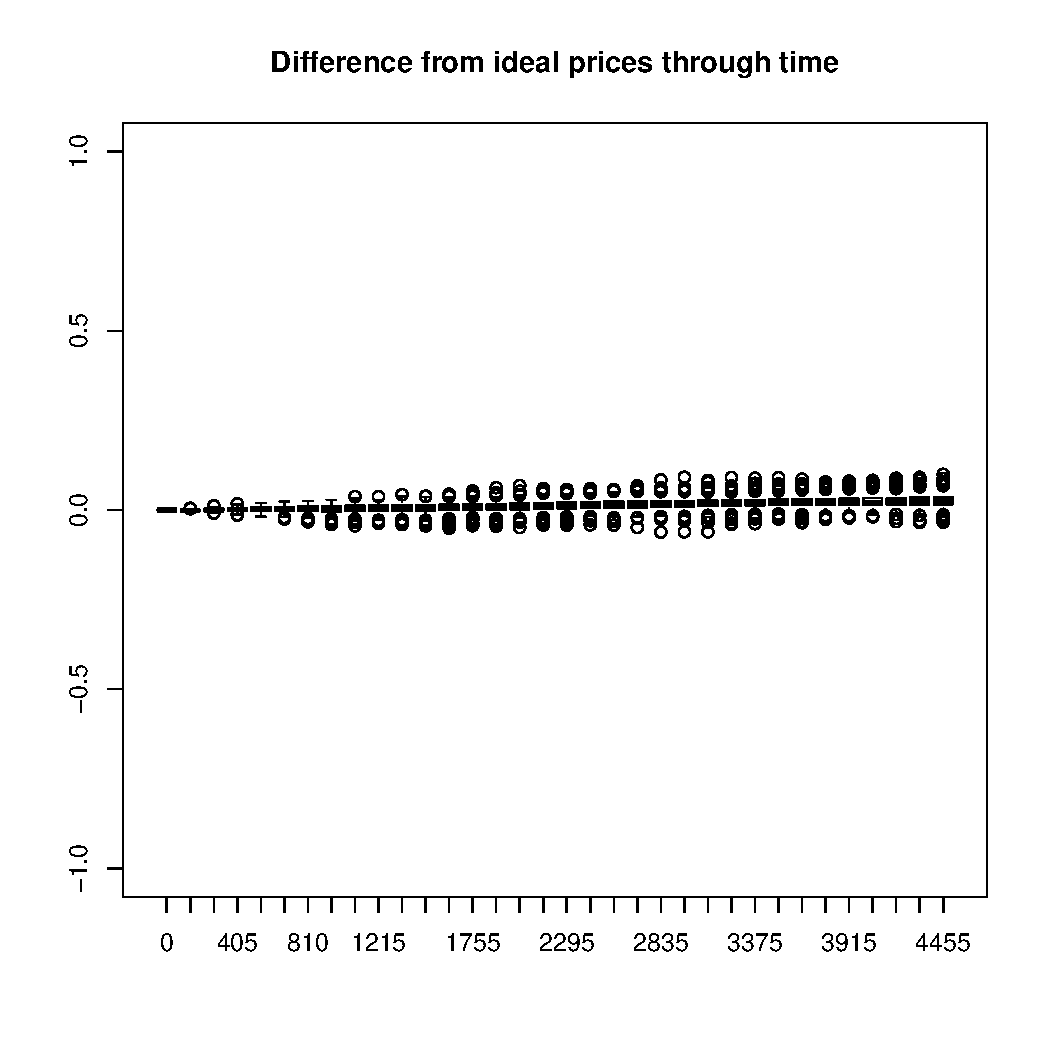
\includegraphics[width=.18\textwidth]{/home/scarrign/projects/PhD/doc/thesis/images/Prices-3_cult-prod_init-man_volsel-gino_ufun-cust.pdf} & \includegraphics[width=.18\textwidth]{/home/scarrign/projects/PhD/doc/thesis/images/Quantities-3_cult-prod_init-man_volsel-gino_ufun-cust.pdf} \\ 
  prod & man & gino & gin & 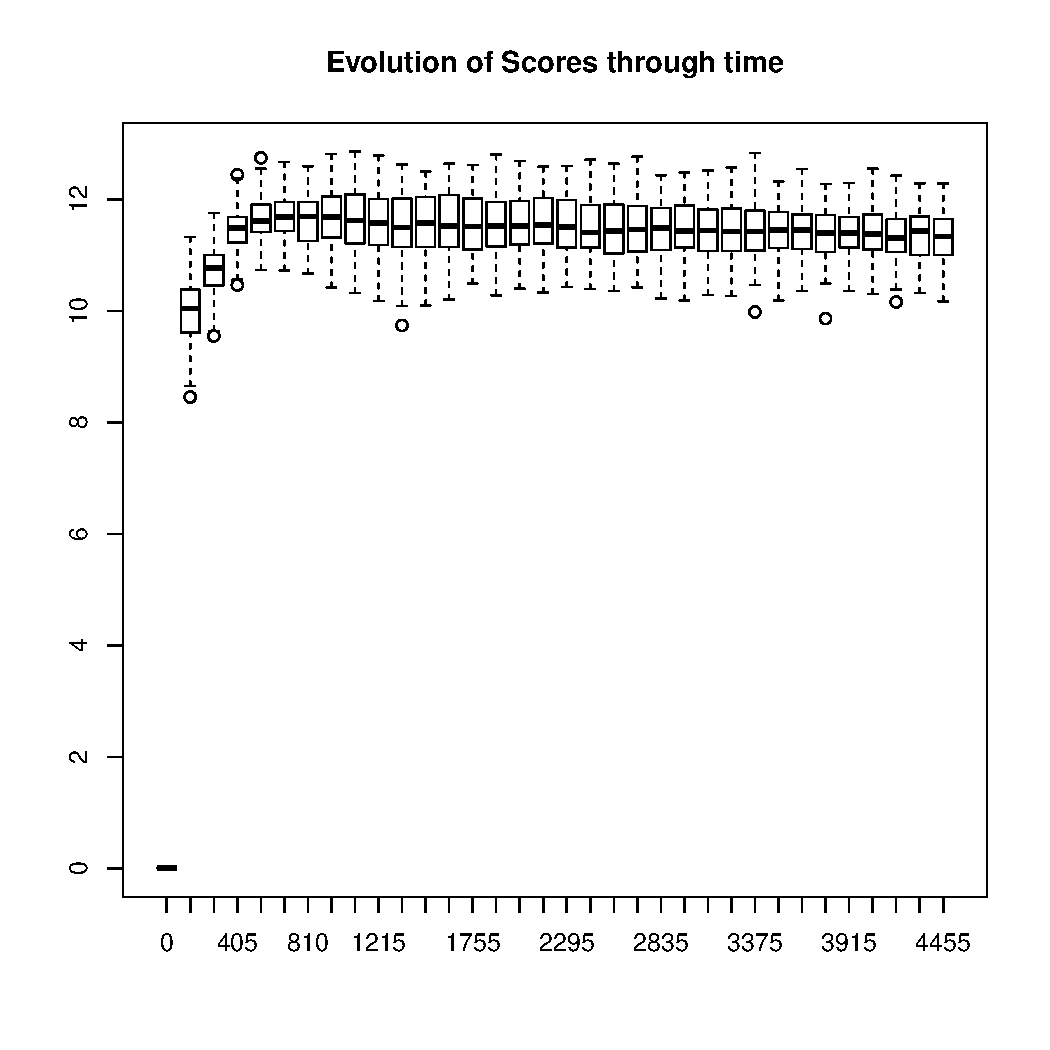
\includegraphics[width=.18\textwidth]{/home/scarrign/projects/PhD/doc/thesis/images/Scores-4_cult-prod_init-man_volsel-gino_ufun-gin.pdf} & \includegraphics[width=.18\textwidth]{/home/scarrign/projects/PhD/doc/thesis/images/Prices-4_cult-prod_init-man_volsel-gino_ufun-gin.pdf} & 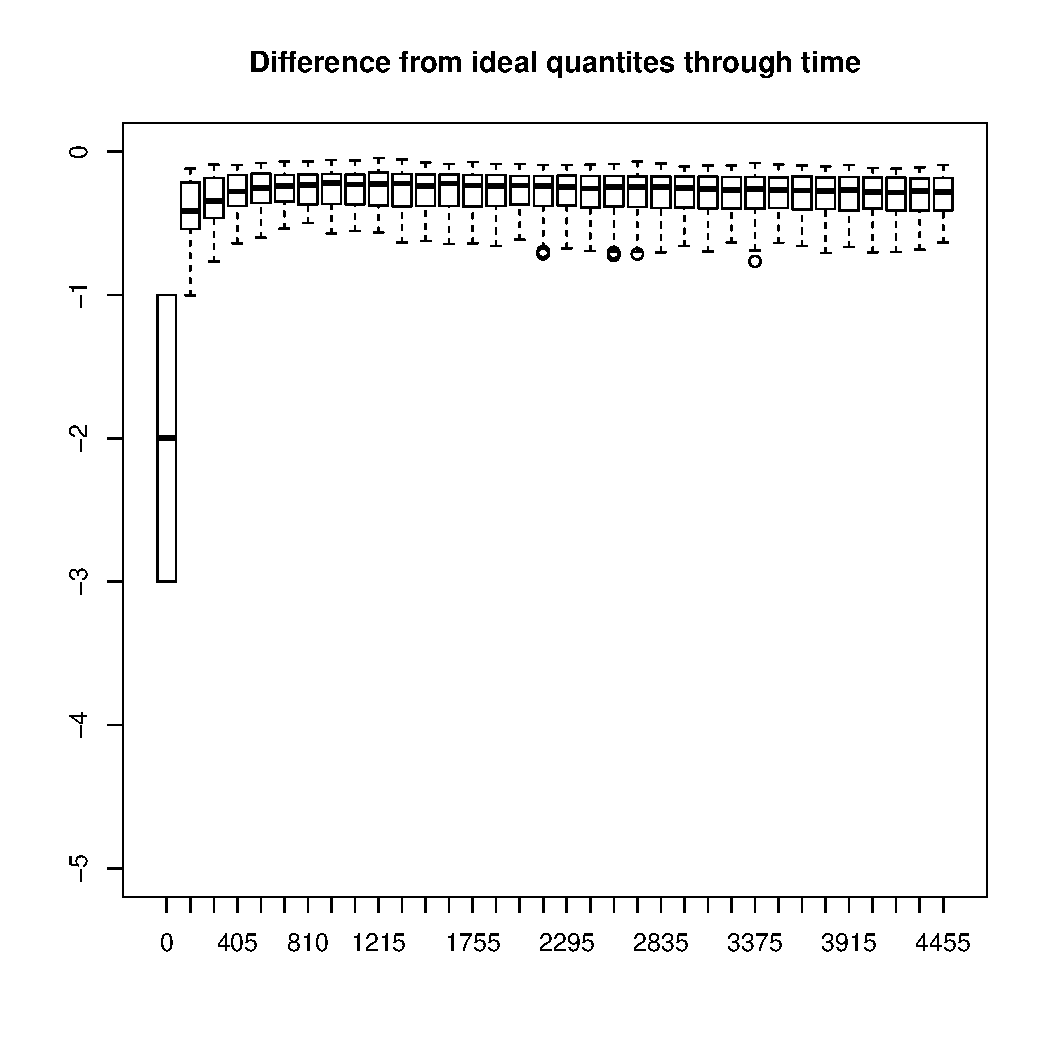
\includegraphics[width=.18\textwidth]{/home/scarrign/projects/PhD/doc/thesis/images/Quantities-4_cult-prod_init-man_volsel-gino_ufun-gin.pdf} \\ 
   \hline
\end{tabular}
\end{table}

\begin{table}[ht]
\centering
\begin{tabular}{lllllll}
  \hline
Copy & Init & Choice & Util & Scores & Prices & Quantities \\ 
  \hline
  prod & rand & gin & cust & 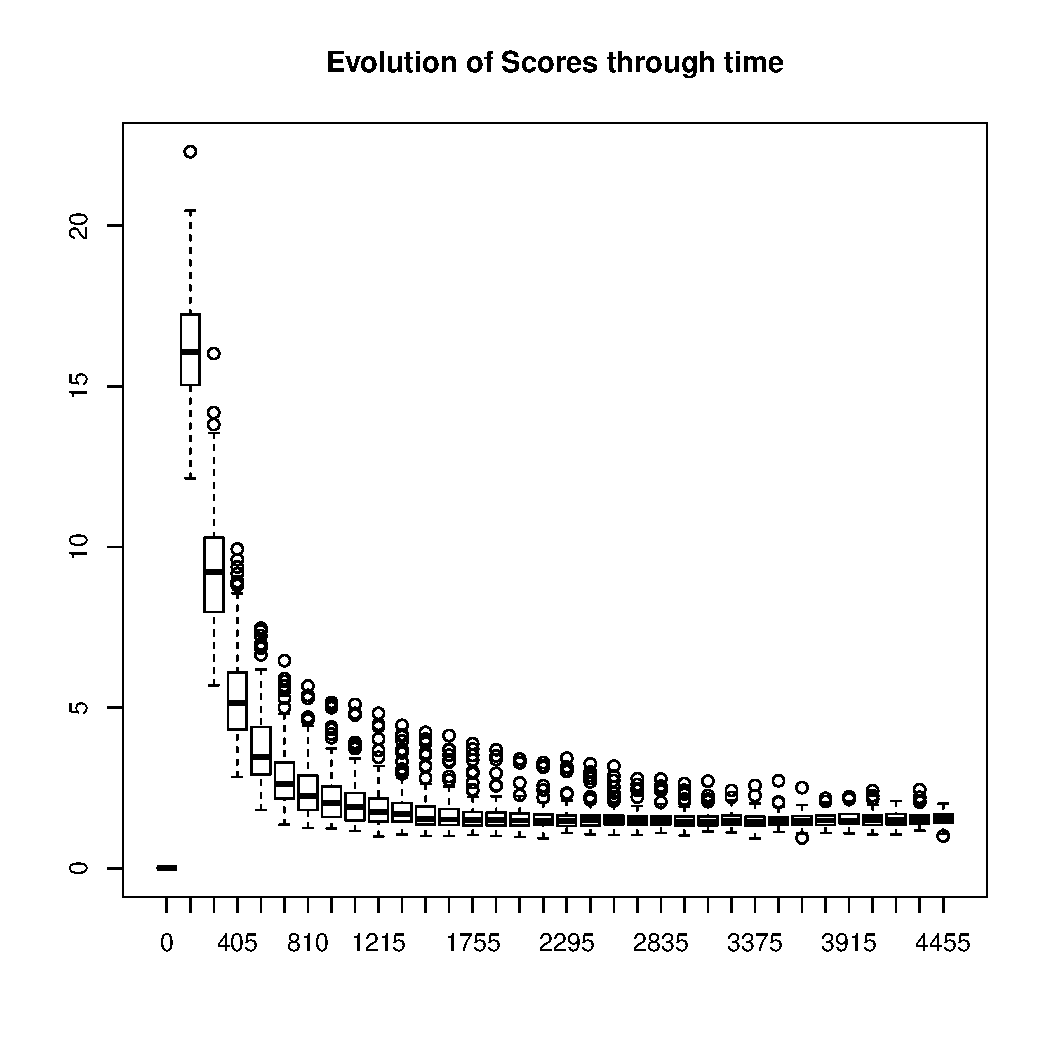
\includegraphics[width=.18\textwidth]{/home/scarrign/projects/PhD/doc/thesis/images/Scores-5_cult-prod_init-rand_volsel-gin_ufun-cust.pdf} & \includegraphics[width=.18\textwidth]{/home/scarrign/projects/PhD/doc/thesis/images/Prices-5_cult-prod_init-rand_volsel-gin_ufun-cust.pdf} & \includegraphics[width=.18\textwidth]{/home/scarrign/projects/PhD/doc/thesis/images/Quantities-5_cult-prod_init-rand_volsel-gin_ufun-cust.pdf} \\ 
  prod & rand & gin & gin & \includegraphics[width=.18\textwidth]{/home/scarrign/projects/PhD/doc/thesis/images/Scores-6_cult-prod_init-rand_volsel-gin_ufun-gin.pdf} & \includegraphics[width=.18\textwidth]{/home/scarrign/projects/PhD/doc/thesis/images/Prices-6_cult-prod_init-rand_volsel-gin_ufun-gin.pdf} & 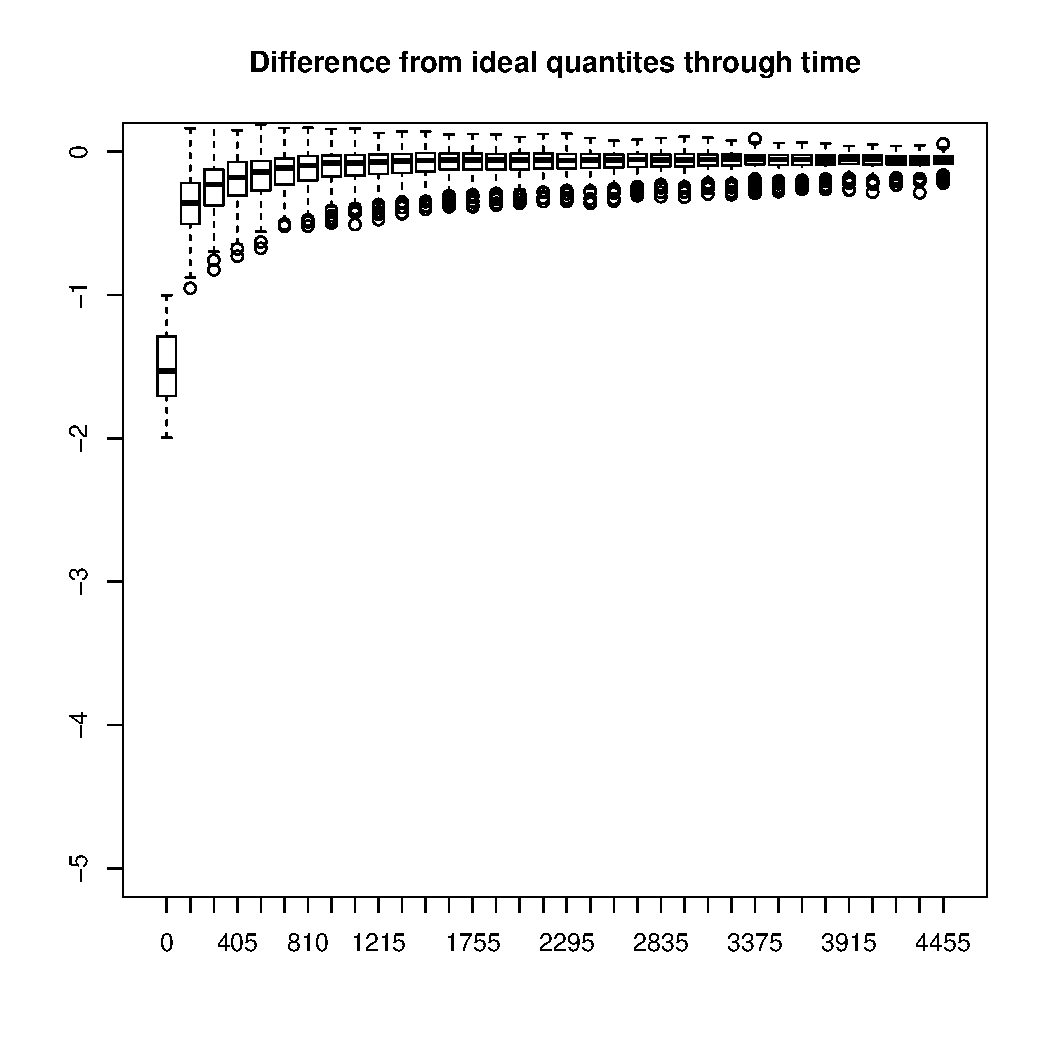
\includegraphics[width=.18\textwidth]{/home/scarrign/projects/PhD/doc/thesis/images/Quantities-6_cult-prod_init-rand_volsel-gin_ufun-gin.pdf} \\ 
  prod & rand & gino & cust & \includegraphics[width=.18\textwidth]{/home/scarrign/projects/PhD/doc/thesis/images/Scores-7_cult-prod_init-rand_volsel-gino_ufun-cust.pdf} & \includegraphics[width=.18\textwidth]{/home/scarrign/projects/PhD/doc/thesis/images/Prices-7_cult-prod_init-rand_volsel-gino_ufun-cust.pdf} & \includegraphics[width=.18\textwidth]{/home/scarrign/projects/PhD/doc/thesis/images/Quantities-7_cult-prod_init-rand_volsel-gino_ufun-cust.pdf} \\ 
  prod & rand & gino & gin & \includegraphics[width=.18\textwidth]{/home/scarrign/projects/PhD/doc/thesis/images/Scores-8_cult-prod_init-rand_volsel-gino_ufun-gin.pdf} & \includegraphics[width=.18\textwidth]{/home/scarrign/projects/PhD/doc/thesis/images/Prices-8_cult-prod_init-rand_volsel-gino_ufun-gin.pdf} & \includegraphics[width=.18\textwidth]{/home/scarrign/projects/PhD/doc/thesis/images/Quantities-8_cult-prod_init-rand_volsel-gino_ufun-gin.pdf} \\ 
   \hline
\end{tabular}
\end{table}

\begin{table}[ht]
\centering
\begin{tabular}{lllllll}
  \hline
Copy & Init & Choice & Util & Scores & Prices & Quantities \\ 
  \hline
  prod & randn & gin & cust & \includegraphics[width=.18\textwidth]{/home/scarrign/projects/PhD/doc/thesis/images/Scores-9_cult-prod_init-randn_volsel-gin_ufun-cust.pdf} & \includegraphics[width=.18\textwidth]{/home/scarrign/projects/PhD/doc/thesis/images/Prices-9_cult-prod_init-randn_volsel-gin_ufun-cust.pdf} & \includegraphics[width=.18\textwidth]{/home/scarrign/projects/PhD/doc/thesis/images/Quantities-9_cult-prod_init-randn_volsel-gin_ufun-cust.pdf} \\ 
  prod & randn & gin & gin & \includegraphics[width=.18\textwidth]{/home/scarrign/projects/PhD/doc/thesis/images/Scores-10_cult-prod_init-randn_volsel-gin_ufun-gin.pdf} & \includegraphics[width=.18\textwidth]{/home/scarrign/projects/PhD/doc/thesis/images/Prices-10_cult-prod_init-randn_volsel-gin_ufun-gin.pdf} & \includegraphics[width=.18\textwidth]{/home/scarrign/projects/PhD/doc/thesis/images/Quantities-10_cult-prod_init-randn_volsel-gin_ufun-gin.pdf} \\ 
  prod & randn & gino & cust & \includegraphics[width=.18\textwidth]{/home/scarrign/projects/PhD/doc/thesis/images/Scores-11_cult-prod_init-randn_volsel-gino_ufun-cust.pdf} & \includegraphics[width=.18\textwidth]{/home/scarrign/projects/PhD/doc/thesis/images/Prices-11_cult-prod_init-randn_volsel-gino_ufun-cust.pdf} & \includegraphics[width=.18\textwidth]{/home/scarrign/projects/PhD/doc/thesis/images/Quantities-11_cult-prod_init-randn_volsel-gino_ufun-cust.pdf} \\ 
  prod & randn & gino & gin & \includegraphics[width=.18\textwidth]{/home/scarrign/projects/PhD/doc/thesis/images/Scores-12_cult-prod_init-randn_volsel-gino_ufun-gin.pdf} & \includegraphics[width=.18\textwidth]{/home/scarrign/projects/PhD/doc/thesis/images/Prices-12_cult-prod_init-randn_volsel-gino_ufun-gin.pdf} & \includegraphics[width=.18\textwidth]{/home/scarrign/projects/PhD/doc/thesis/images/Quantities-12_cult-prod_init-randn_volsel-gino_ufun-gin.pdf} \\ 
   \hline
\end{tabular}
\end{table}

\begin{table}[ht]
\centering
\begin{tabular}{lllllll}
  \hline
Copy & Init & Choice & Util & Scores & Prices & Quantities \\ 
  \hline
  integ & man & gin & cust & \includegraphics[width=.18\textwidth]{/home/scarrign/projects/PhD/doc/thesis/images/Scores-13_cult-integ_init-man_volsel-gin_ufun-cust.pdf} & \includegraphics[width=.18\textwidth]{/home/scarrign/projects/PhD/doc/thesis/images/Prices-13_cult-integ_init-man_volsel-gin_ufun-cust.pdf} & \includegraphics[width=.18\textwidth]{/home/scarrign/projects/PhD/doc/thesis/images/Quantities-13_cult-integ_init-man_volsel-gin_ufun-cust.pdf} \\ 
  integ & man & gin & gin & \includegraphics[width=.18\textwidth]{/home/scarrign/projects/PhD/doc/thesis/images/Scores-14_cult-integ_init-man_volsel-gin_ufun-gin.pdf} & \includegraphics[width=.18\textwidth]{/home/scarrign/projects/PhD/doc/thesis/images/Prices-14_cult-integ_init-man_volsel-gin_ufun-gin.pdf} & \includegraphics[width=.18\textwidth]{/home/scarrign/projects/PhD/doc/thesis/images/Quantities-14_cult-integ_init-man_volsel-gin_ufun-gin.pdf} \\ 
  %integ & man & gino & cust & \includegraphics[width=.18\textwidth]{/home/scarrign/projects/PhD/doc/thesis/images/Scores-15_cult-integ_init-man_volsel-gino_ufun-cust.pdf} & \includegraphics[width=.18\textwidth]{/home/scarrign/projects/PhD/doc/thesis/images/Prices-15_cult-integ_init-man_volsel-gino_ufun-cust.pdf} & \includegraphics[width=.18\textwidth]{/home/scarrign/projects/PhD/doc/thesis/images/Quantities-15_cult-integ_init-man_volsel-gino_ufun-cust.pdf} \\ 
  %integ & man & gino & gin & \includegraphics[width=.18\textwidth]{/home/scarrign/projects/PhD/doc/thesis/images/Scores-16_cult-integ_init-man_volsel-gino_ufun-gin.pdf} & \includegraphics[width=.18\textwidth]{/home/scarrign/projects/PhD/doc/thesis/images/Prices-16_cult-integ_init-man_volsel-gino_ufun-gin.pdf} & \includegraphics[width=.18\textwidth]{/home/scarrign/projects/PhD/doc/thesis/images/Quantities-16_cult-integ_init-man_volsel-gino_ufun-gin.pdf} \\ 
   \hline
\end{tabular}
\end{table}

\begin{table}[ht]
\centering
\begin{tabular}{lllllll}
  \hline
Copy & Init & Choice & Util & Scores & Prices & Quantities \\ 
  \hline
  integ & rand & gin & cust & \includegraphics[width=.18\textwidth]{/home/scarrign/projects/PhD/doc/thesis/images/Scores-17_cult-integ_init-rand_volsel-gin_ufun-cust.pdf} & \includegraphics[width=.18\textwidth]{/home/scarrign/projects/PhD/doc/thesis/images/Prices-17_cult-integ_init-rand_volsel-gin_ufun-cust.pdf} & \includegraphics[width=.18\textwidth]{/home/scarrign/projects/PhD/doc/thesis/images/Quantities-17_cult-integ_init-rand_volsel-gin_ufun-cust.pdf} \\ 
  integ & rand & gin & gin & \includegraphics[width=.18\textwidth]{/home/scarrign/projects/PhD/doc/thesis/images/Scores-18_cult-integ_init-rand_volsel-gin_ufun-gin.pdf} & \includegraphics[width=.18\textwidth]{/home/scarrign/projects/PhD/doc/thesis/images/Prices-18_cult-integ_init-rand_volsel-gin_ufun-gin.pdf} & \includegraphics[width=.18\textwidth]{/home/scarrign/projects/PhD/doc/thesis/images/Quantities-18_cult-integ_init-rand_volsel-gin_ufun-gin.pdf} \\ 
  integ & rand & gino & cust & \includegraphics[width=.18\textwidth]{/home/scarrign/projects/PhD/doc/thesis/images/Scores-19_cult-integ_init-rand_volsel-gino_ufun-cust.pdf} & \includegraphics[width=.18\textwidth]{/home/scarrign/projects/PhD/doc/thesis/images/Prices-19_cult-integ_init-rand_volsel-gino_ufun-cust.pdf} & \includegraphics[width=.18\textwidth]{/home/scarrign/projects/PhD/doc/thesis/images/Quantities-19_cult-integ_init-rand_volsel-gino_ufun-cust.pdf} \\ 
  integ & rand & gino & gin & \includegraphics[width=.18\textwidth]{/home/scarrign/projects/PhD/doc/thesis/images/Scores-20_cult-integ_init-rand_volsel-gino_ufun-gin.pdf} & \includegraphics[width=.18\textwidth]{/home/scarrign/projects/PhD/doc/thesis/images/Prices-20_cult-integ_init-rand_volsel-gino_ufun-gin.pdf} & \includegraphics[width=.18\textwidth]{/home/scarrign/projects/PhD/doc/thesis/images/Quantities-20_cult-integ_init-rand_volsel-gino_ufun-gin.pdf} \\ 
   \hline
\end{tabular}
\end{table}

\begin{table}[ht]
\centering
\begin{tabular}{lllllll}
  \hline
Copy & Init & Choice & Util & Scores & Prices & Quantities \\ 
  \hline
  integ & randn & gin & cust & \includegraphics[width=.18\textwidth]{/home/scarrign/projects/PhD/doc/thesis/images/Scores-21_cult-integ_init-randn_volsel-gin_ufun-cust.pdf} & \includegraphics[width=.18\textwidth]{/home/scarrign/projects/PhD/doc/thesis/images/Prices-21_cult-integ_init-randn_volsel-gin_ufun-cust.pdf} & \includegraphics[width=.18\textwidth]{/home/scarrign/projects/PhD/doc/thesis/images/Quantities-21_cult-integ_init-randn_volsel-gin_ufun-cust.pdf} \\ 
  integ & randn & gin & gin & \includegraphics[width=.18\textwidth]{/home/scarrign/projects/PhD/doc/thesis/images/Scores-22_cult-integ_init-randn_volsel-gin_ufun-gin.pdf} & \includegraphics[width=.18\textwidth]{/home/scarrign/projects/PhD/doc/thesis/images/Prices-22_cult-integ_init-randn_volsel-gin_ufun-gin.pdf} & \includegraphics[width=.18\textwidth]{/home/scarrign/projects/PhD/doc/thesis/images/Quantities-22_cult-integ_init-randn_volsel-gin_ufun-gin.pdf} \\ 
  integ & randn & gino & cust & \includegraphics[width=.18\textwidth]{/home/scarrign/projects/PhD/doc/thesis/images/Scores-23_cult-integ_init-randn_volsel-gino_ufun-cust.pdf} & \includegraphics[width=.18\textwidth]{/home/scarrign/projects/PhD/doc/thesis/images/Prices-23_cult-integ_init-randn_volsel-gino_ufun-cust.pdf} & \includegraphics[width=.18\textwidth]{/home/scarrign/projects/PhD/doc/thesis/images/Quantities-23_cult-integ_init-randn_volsel-gino_ufun-cust.pdf} \\ 
  integ & randn & gino & gin & \includegraphics[width=.18\textwidth]{/home/scarrign/projects/PhD/doc/thesis/images/Scores-24_cult-integ_init-randn_volsel-gino_ufun-gin.pdf} & \includegraphics[width=.18\textwidth]{/home/scarrign/projects/PhD/doc/thesis/images/Prices-24_cult-integ_init-randn_volsel-gino_ufun-gin.pdf} & \includegraphics[width=.18\textwidth]{/home/scarrign/projects/PhD/doc/thesis/images/Quantities-24_cult-integ_init-randn_volsel-gino_ufun-gin.pdf} \\ 
   \hline
\end{tabular}
\end{table}


\section{Money}
While putting moeny I discovered that I can jsut remove the test of the counter trade: it prevents numerous trade to be achieved while it should not => by looking at what was responsible of almost 1/third of the failed trades.
\end{document}

